
% JuliaCon proceedings template
\documentclass{juliacon}
\setcounter{page}{1}

\begin{document}

% **************GENERATED FILE, DO NOT EDIT**************

\title{My JuliaCon proceeding}

\author[1]{1st author}
\author[1, 2]{2nd author}
\author[2]{3rd author}
\affil[1]{University}
\affil[2]{National Lab}

\keywords{Julia, Optimization, Game theory, Compiler}

\hypersetup{
pdftitle = {My JuliaCon proceeding},
pdfsubject = {JuliaCon 2022 Proceedings},
pdfauthor = {1st author, 2nd author, 3rd author},
pdfkeywords = {Julia, Optimization, Game theory, Compiler},
}



\maketitle

\begin{abstract}

\verb|AdaptiveHierarchicalRegularBinning.jl| computes a hierarchical space-partitioning
tree for a given set of points of arbitrary dimensions, that divides the space and
stores the reordered points offering efficient access. Space-partitioning data
structures are vital for algorithms that exploit spatial distance to reduce
computational complexity, see for example the Fast Multipole Method, and algorithms
finding nearest neighbors and their applications.

\end{abstract}


\section{Motivation}
Space partitioning algorithms play a pivotal role in improving the runtime
performance of computational algorithms by dividing data into smaller,
manageable sections. These algorithms are designed to optimize the performance
of computational algorithms by efficiently partitioning the data space in a
manner that aligns with the specific requirements of the problem domain.
\\\\
In this section, we delve into the need for space partitioning
algorithms and their significance in addressing the computational bottlenecks
faced by certain algorithms. We examine three prominent application domains:
k-nearest neighbors (kNN) search, collision detection, and the fast multipole
method (FMM). These domains represent scenarios where the all-vs-all model,
involving computations between every pair of data points, hampers the runtime
performance of algorithms.

\subsection{kNN}
One common challenge encountered in computational algorithms, such as k-nearest
neighbors (kNN) search, is the need to compute distances between each pair of
points in the data space. This all-vs-all model becomes computationally
expensive as the dataset size increases. However, by employing a space
partitioning algorithm, the number of distance computations can be
significantly reduced. Instead of calculating distances between all points,
the algorithm subdivides the space into smaller sections, enabling the
identification of nearest neighbors within localized partitions. This approach
drastically improves the runtime performance of the kNN algorithm by reducing
the computational burden associated with distance calculations.

\subsection{Collision Detection}
Collision detection algorithms also stand to benefit from space
partitioning techniques. In scenarios where it is necessary to determine if a
collision occurs between objects in a $d$-dimensional space, the all-vs-all
model becomes impractical for large-scale simulations. By partitioning the
space into smaller regions or bins, collision detection algorithms can focus
computations solely on objects within the same partition. This significantly
reduces the number of pairwise collision checks required and provides a
substantial performance improvement in terms of runtime. Specific space
partitioning algorithms enable efficient identification of potential collision
candidates, contributing to faster and more accurate collision detection in
simulations and virtual environments.

\subsection{FMM}

The fast multipole method (FMM), explored in \cite{FMM} and \cite{AMM}, is an
important algorithm used for solving the N-body problem, which involves the
interaction of multiple particles in a system. The traditional implementation
of FMM suffers from a high computational complexity, as it requires pairwise
computations between all particles in the system. However, space partitioning
algorithms offer an opportunity to optimize the FMM by dividing the space into
subregions or bins. By employing space partitioning techniques, the FMM
algorithm can efficiently identify distant interactions, reducing the number of
pairwise computations required and significantly improving the overall runtime
performance. The incorporation of space partitioning algorithms in FMM enables
the efficient solution of the N-body problem and opens doors for the simulation
of large-scale physical systems.



\section{Implementation}
The partitioning of a $d$-dimensionsional cloud of points is a fundamental task
in many computational applications. The
\verb|AdaptiveHierarchicalRegularBinning.jl|
algorithm offers an effective approach to address this challenge. By utilizing
the Morton curve, a type of one-dimensional space filling curve, this algorithm
maps each point from the $d$-dimensional space to a one-dimensional
representation. Consequently, the hierarchical tree structure is established
based on the Morton index assigned to each point.
\\\\
The \verb|AdaptiveHierarchicalRegularBinning.jl| algorithm leverages the
inherent properties of the Morton curve to efficiently partition the cloud of
points. The Morton curve exhibits a desirable characteristic of spatial
locality preservation, where nearby points in the original $d$-dimensional
space tend to have adjacent Morton indices in the one-dimensional space. This
property ensures that points with similar spatial coordinates are grouped
together in the resulting hierarchical tree structure.

\subsection{Morton encoding}
Morton indices are binary words grouped into $l$ levels of $d$ bits each. Each level
describes in an increasingly finer detail the area in which the point resides. The
first level, comprised of the $d$ most significant bits of the morton index, describes
only in which half of each dimension the point lies.

$$b = \left\{\begin{matrix}
  (0)_2, & \textrm{Left-most half}  \\
  (1)_2, & \textrm{Right-most half}
\end{matrix}\right.$$


\begin{definition}[Left/Right-mostness]
  For a $1$-dimensional simply connected space $A = [m, M)$, we say that
  $x$ lies in the Left-most half, if and only if, $x<h=\frac{M+m}{2}$.
  Otherwise $x$ lies in the Right-most half.

  $$
  \begin{matrix}
    L &\triangleq& [m, h) \\
    R &\triangleq& [h, M)
  \end{matrix}
  $$
\end{definition}


\begin{example}[Morton index interpretation]
  Figure \ref{spatial-tree} depicts a $2$-dimensional space and a target spatial
  tree of at most $2$ levels (other than the root). The morton index, in such a tree,
  will have a length of $2\cdot2=4$. Assume we compute a morton index of $(0011)_2$.
  The first group is comprised of the $2$ most significant bits and addresses the first
  level of the tree (the one directly under root).
  \\\\
  The most significant bit addresses the first dimension and the second most significant
  bit addresses the second dimension. The value $(0)_2$ signifies that the point lies in
  the left-most half of each dimension.
  \\\\
  The next group describes the same quantities only a level lower. Left/Right-mostness
  is defined in the context of that level. Both values are $(1)_2$ so the point lies in
  the right-most half of both dimensions in the second level.
  \\\\
  Summarizing, the point belongs to the:
  \begin{itemize}
    \item right-most half of the left-most half of the first dimension.
    \item right-most half of the left-most half of the second dimension.
  \end{itemize}

  \begin{figure}[!ht]
    \centerline{
      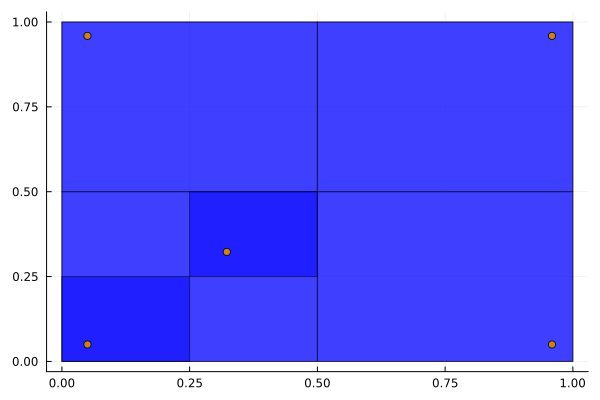
\includegraphics[width=10pc]{figures/spatial-division.png}
      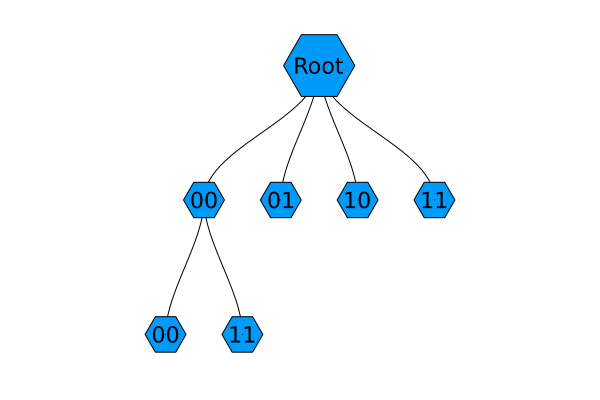
\includegraphics[width=10pc]{figures/spatial-tree.png}
    }
    \caption{ (a) Spatial division, (b) Spatial tree }
    \label{spatial-tree}
  \end{figure}
\end{example}

\subsection{Reordering}
Sorting the points based on their Morton indices is a key operation in the
\verb|AdaptiveHierarchicalRegularBinning.jl| algorithm, enabling efficient
access during tree iteration. To achieve this, the algorithm employs the
\verb|MSD Radixsort| \cite{radixsort} algorithm, or Most Significant Digit
Radixsort, which examines the most significant bits of the Morton indices. By
grouping points with similar prefixes together, the sorted order achieved
through \verb|MSD Radixsort| enhances data locality and improves performance.
This arrangement ensures that neighboring points in the original $d$-dimensional
space are adjacent in the sorted sequence, optimizing point retrieval and
overall algorithm efficiency.

\subsubsection{MSD Radixsort}
\verb|MSD Radixsort| sorts based on the most significant radix. Afterwards, elements
with the same most significant digit (MSD) form a consecutive sub-array. The algorithm
recurses for each such sub-array selecting the next digit in line, leading to
$O(n\cdot m)$ runtime complexity, where $n$ is the size of the array and $m$ is
the number of recursions. Selecting a large radix is crucial for the algorithm
since a large radix lowers the number of recursions.
\\\\
\verb|MSD Radixsort| respects the hierarchical nature of the target tree and thus it offers
benefits over other sorting algorithms. Each recursion of the algorithm sorts a section
of the resulting tree. If the radix matches the number of dimensions then each recursion
sorts the current level of the tree.
\\\\
When the number of elements of a sub array is small the recursion for that sub-array stops.
This leads to a partialy sorted array by design. Not sorting small sub-arrays leads to less
overhead without sacrificing future performance. Nodes with unsorted morton indices will
always be leaf nodes.
\\\\
\verb|MSD Radixsort| can be trivialy parallelized. After the initial sorting, the formed
sub-arrays are mutually exclusive, meaning that no data dependencies are shared between
them. Each sub-array can then be sorted in parallel.

\subsubsection{Countsort}
\verb|MSD Radixsort| needs a sorting algorithm to sort the selected radix in each recursion.
\verb|Countsort| is a great fit for this type of sorting. \verb|Countsort| trades
space complexity for runtime complexity. The algorithm uses an auxilary vector, whose
size scales linearly with the selected radix $O(r)$. The benefit is the runtime
complexity is order $O(n + r)$ where $n$ is the size of the array to sort. Typically, $n \gg r$
and so the runtime complexity reduces to $O(n)$.
\\\\
\verb|Countsort| can be parallelized as well, though not as trivialy. The parallel version
of \verb|Countsort| requires space complexity of $O(t\cdot r)$ and runtime complexity of
$O(n/t + t\cdot r)$ where $t$ is the number of threads in the system. As long as $n$ is
sufficiently large $n \gg t^2\cdot r$ then the parallel implementation is preferable since
the runtime complexity reduces to $O(n/t)$.

\subsubsection{Radix trade-off}
While \verb|MSD Radixsort| fairs better for larger radices, \verb|Countsort| reduces in
performance.

\begin{example}
  For a $128$-bit morton index, a radix of $16$-bits is selected.
  The number of recursions in this case is $8$ which is fairly small and the condition
  $n\gg t^2\cdot r$ can still be satisfied.
  % TODO: Graphs runtime complexity vs r
\end{example}

Our implementation utilizes a watefall scheme to adapt to the needs of the problem at
hand. There are three different thresholds that can tune the runtime performance of the
spatial partitioning.

\begin{itemize}
  \item \verb|Huge| threshold
  \item \verb|Big| threshold
  \item \verb|Small| threshold
\end{itemize}

$$ \textrm{Huge} > \textrm{Big} > \textrm{Small} $$

For sub-arrays that are larger than the \verb|Huge| threshold our implementation
uses parallel \verb|MSD Radixsort|, otherwise it falls back to the non parallel variant.
\\\\
For sub-arrays that are larger than the \verb|Big| threshold our implementation uses
parallel \verb|Countsort|, otherwise it falls back to the non parallel variant.
\\\\
For sub-arrays that are smaller than the \verb|Small| threshold our implementation
stops the recursion of \verb|MSD Radixsort|.


\subsection{Tree}
The resulting tree is memory-dense, meaning that it does not store empty nodes.
The root node encapsulates the entire cloud of points, while each child node points to
a consecutive sub-array of those points. This characteristic holds true for every node
within the tree. Each node is also aware if its level, parent and children.


\section{Usage}

\begin{lstlisting}[language = Bash]
  $ julia -t auto
\end{lstlisting}

\begin{lstlisting}[language = Julia]
  using AdaptiveHierarchicalRegularBinning
  n = 10000
  d = 5
  X = rand(n, d)

  tree = regular_bin(X, dpt, sml_th; dims=2)
  # X is no permuted to accomodate morton encoding

  for leaf in Leaves(tree)
  # iterates over the tree's leafs
  end

  for node in PreOrderDFS(tree)
    # iterates over the tree's nodes in pre order
  end

  I, D = knn(tree, X)

  original_perm!(tree, I, D)
  # I and D are now refering to the
  # original permutation
\end{lstlisting}


\section{Theory}
Assuming a set of $n$ $d$-dimensional points $\mathcal{V}$, we represent $\mathcal{V}$ as
the $d \times n$ matrix $V$. \verb|AdaptiveHierarchicalRegularBinning.jl| uses Morton
encoding to map each $d$-dimenensional point of $\mathcal{V}$ to a $1$-dimenensional
space filling curve, Z-order curve.
\\\\
The mapping proccess requires 3 distinct steps.

\begin{itemize}
  \item Normalize $\mathcal{V}$ such that each vector $\vec{v}$ of $\mathcal{V}$
  satisfies $\vec{v} \in [0,1)^d$.
  \item Quantize each dimension using an $l$-bit quantizer, where $l$ is the maximum
  depth of the target tree.
  \item Bit-interleave the output of the quantizer.
\end{itemize}

\subsection{Normalization}
In order to compute the hierarchical tree we first normalize $\mathcal{V}$.

$$ \vec{v} \in \mathcal{H}, \forall \vec{v} \in \mathcal{V}$$

Where $\mathcal{H}$ is the connected $d$-dimensional space that contains all vectors
of $\mathcal{V}$.

$$ H \triangleq [m_1, M_1] \times [m_2, M_2] \times \cdots \times [m_d, M_d] $$

Where
$$\space m_i = \min_j\left(V_{i,j}\right), \forall i \in \left\{1, 2, \cdots, d\right\}$$
$$\space M_i = \max_j\left(V_{i,j}\right), \forall i \in \left\{1, 2, \cdots, d\right\}$$

Therefore the goal of the normalization process is to define a $1-1$ function $\hat{f}$
such that

$$\hat{f}: \mathcal{H} \rightarrow [0, 1)^d$$

Applying the function to each element of $\mathcal{V}$ defines a new set of points
$\hat{\mathcal{V}}$ the elements of which are by definition inside a $d$-dimensional unit
hypercube.

$$ \hat{\mathcal{V}} \triangleq \left\{ \hat{f}\left(v\right) : v \in \mathcal{V} \right\}  $$
$$ \vec{v} \in [0, 1)^d, \forall \vec{v} \in \hat{\mathcal{V}} $$

Furthermore, the function $\hat{f}$ must satisfy an additional property, namely,
the preservation of relative distances.

$$ ||\vec{v_1} - \vec{v_2}|| \geq ||\vec{v_1} - \vec{v_3}|| \Leftrightarrow ||\hat{f}(\vec{v_1}) - \hat{f}(\vec{v_2})|| \geq ||\hat{f}(\vec{v_1}) - \hat{f}(\vec{v_3})||$$
$$ \forall \vec{v_1}, \vec{v_2}, \vec{v_3} \in \mathcal{V} $$

Given this constraint we can therefore define the function $\hat{f}$ as such
\begin{definition}
  $$\hat{f}(\vec{v}) \triangleq \frac{\vec{v} - \vec{t}}{s}, \forall \vec{v} \in \mathcal{H} \quad \textrm{where}\; \vec{t} \in \mathbb{R}^d, s\in\mathbb{R}^*$$
\end{definition}

It can be proven that this definition satisfies the constraint

\begin{lemma}
  $$
  \begin{matrix}
    ||\hat{f}(\vec{v_1}) - \hat{f}(\vec{v_2})|| &=& || \frac{\vec{v_1} - \vec{t}}{s} - \frac{\vec{v_2} - \vec{t}}{s}||\\
                                                &=& || \frac{\vec{v_1} - \vec{t} - \vec{v_2} + \vec{t}}{s}||\\
                                                &=& || \frac{\vec{v_1} - \vec{v_2}}{s}||\\
                                                &\triangleq& \frac{||\vec{v_1} - \vec{v_2}||}{|s|} & \forall v_1, v_2 \in \mathcal{V}\\
  \end{matrix}
  $$
\end{lemma}
\begin{proof}
  $$
  \begin{matrix}
    ||\hat{f}(\vec{v_1}) - \hat{f}(\vec{v_2})|| \geq ||\hat{f}(\vec{v_1}) - \hat{f}(\vec{v_3})|| &\Leftrightarrow&\\
    \frac{||\vec{v_1} - \vec{v_2}||}{|s|} \geq \frac{||\vec{v_1} - \vec{v_3}||}{|s|} &\Leftrightarrow&\\
    ||\vec{v_1} - \vec{v_2}|| \geq ||\vec{v_1} - \vec{v_3}||
  \end{matrix}
  $$
$$$$
\end{proof}

We require the image of $\hat{f}$ to be $\hat{f}(\mathcal{H}) = [0,1)^d$. Thus we can
compute $\vec{t}$ and $s$ to satisfy that constraint.

$$
\begin{matrix}
  \hat{f}(\mathcal{H}) & \triangleq & \bigtimes\limits_{i=1}^d [\hat{f}(m_i), \hat{f}(M_i)] &\\
                       & = & \bigtimes\limits_{i=1}^d [\frac{m_i-\vec{t}_i}{s}, \frac{M_i-\vec{t}_i}{s}] &\
\end{matrix}
$$

Hence,

$$ \vec{t}_i = \begin{pmatrix} m_1 \\ m_2 \\ \vdots \\ m_d \end{pmatrix}$$
$$ s = \max_i(M_i-m_i)$$

Therefore $\hat{f}(\mathcal{H}) \subseteq [0, 1]^d \Leftrightarrow \hat{f}: \mathcal{H} \rightarrow [0,1]^d$
\\\\
A subtle, yet crucial modification is made to the computed $s$ in order to
accurately map each dimension to the interval $[0,1)$, rather than the inclusive range
$[0,1]$.

$$ s' = s + \epsilon(s) $$

We define $\epsilon(s)$ as the smallest possible value such that $s + \epsilon(s) > s$.
In the standard real number system, when $s \in \mathbb{R}$, there is no such value,
due to the uncountably infinite nature of $\mathbb{R}$. But computers use finite bits
to represent floating point values and so $\epsilon(s)$ is the machine's epsilon value.

\subsection{Quantization}
We use an $l$-bit quiantizer to quantize $\hat{\mathcal{V}}$.
$$q^{(l)}(x) = \lfloor x \cdot 2^l \rfloor, \forall x \in [0, 1)$$

This trivialy generalizes to $d$ dimensions.
$$\vec{q^{(l)}}(\vec{x}) = \begin{pmatrix}
  q^{(l)}(x_1)\\
  q^{(l)}(x_2)\\
  \vdots \\
  q^{(l)}(x_d)
\end{pmatrix}, \forall \vec{x} \in [0,1)^d$$

Therefore each dimension is mapped to an $l$-bit word. The bits of
this word approximate the location of the point in the given
dimension.
\\\\
The output of the quantizer can be mapped $1-1$ to a value in the
original space $[0,1)$.

$$ \tilde{x}_l = \frac{q^{(l)}(x)}{2^l} $$

Assume that $q^{(l)}(x) = (b_1b_2b_3\dots b_l)_2$ where $b_1$ is the most significant
bit of the output word and $b_l$ the least significant.
$$
\begin{matrix}
  \tilde{x}_l & = & \frac{q^{(l)}(x)}{2^l} \\
              & = & \frac{(b_1b_2b_3\dots b_l)_2}{2^l} \\
              & = & \frac{\sum\limits_{i=1}^{l} b_i \cdot 2^{l-i}}{2^l} \\
              & = & \sum\limits_{i=1}^{l}\frac{b_i \cdot 2^{l-i}}{2^l} \\
              & = & \sum\limits_{i=1}^{l}b_i \cdot 2^{-i} \\
\end{matrix}
$$

So then, each bit controls a diminishing power of $2$. The geometric interpretation of
this is that
\begin{itemize}
  \item The most significant bit indicates in which half the real value lies, $1$
  for the right-most half and $0$ for the left-most.
  \item The second most significant bit indicates the same but for the previously
  selected half's half.
  \item And so on.
\end{itemize}


\subsection{Morton encoding}
Computing the Z-order curve from the output of the quantizer is done via bit-interleaving.
Assuming that for some input $\vec{x}$
$$
\vec{q}^{(l)}(\vec{x}) =
\begin{pmatrix}
  (b_{11}b_{12}b_{13}\dots b_{1l})_2\\
  (b_{21}b_{22}b_{23}\dots b_{2l})_2\\
  \vdots \\
  (b_{d1}b_{d2}b_{d3}\dots b_{dl})_2
\end{pmatrix}
$$

Interleaving the bits would compute the following binary value.

$$(b_{11}b_{21}\dots b_{d1}\quad b_{12}b_{22}\dots b_{d2}\quad \dots \quad b_{1l}b_{2l}\dots b_{dl})_2$$

This binary value is semanticaly divided into $l$ groups of $d$ bits. Each bit in a group
describe the location of the input vector $\vec{x}$ in the respective dimension, the
first bit describes the first dimension, the second bit the second dimension and so on.
Each group of bits describe wether the value is located in the left-most or the
right-most part of the respective level, the first group describe the whole space
$[0,1)^d$, the second group describe the selected half of the first group and so on.

\section{Limitations}

\subsection{Curse of high dimensionality}
Data of high dimensionality exponatialy get sparser as the number of dimensions grow.
The sparser the data the lower the probabilities are for any two points occupying the same
bin.
\\\\
Assuming uniformly distributed $d$-dimensional $n$ points and a target tree of
$l$ levels, the expected number of points per leaf node is $E[n_\textrm{leaf}]$.

$$E[n_\textrm{leaf}] = \frac{n}{2^{l\cdot d}}$$

The expected number of points per leaf node drops exponentialy with $d$. This extends
to most distributions of points since the probability of a point belonging to a node is a
function of the $d$-dimensional area that the node occupies $A^{(d)}_l $.
In the case of uniform distribution the probability is directly proportional
to this area.

$$A^{(d)}_l = 2^{-l \cdot d}$$

In general the area is $A^{(d)}_l = s\cdot 2^{-l \cdot d}$ where $s$ is the scaling factor
of the original space. But since scaling does not affect the relative density of the
points the probability is not affected.

\subsection{Morton word size}
To compute the Z-order curve we first quantize the real values with an $l$-bit
quantizer and then we interleave $d$ words of $l$ bits. The resulting binary value has in
total $l\cdot d$ bits which are stored as an \verb|Unsigned| value, limiting the size of the
value to $128$ bits, which is the biggest \verb|Unsigned| built-in integer.

\subsection{Space complexity}
We perform the partial sorting of the $V$, the cloud of points in an out-of-order fashion,
which marks the space complexity needed for the algorithm as $O(n\cdot d)$ where $n$ is
the number of points and $d$ the number of dimensions. An in-place implementation would
trade-off time complexity for space complexity.


\section{Experiments}
All conducted experiments are executed with a selected radix of $16$ bits and the array
is fully sorted, unless stated otherwise.


\subsection{Runtime performance}
\subsubsection{Scaling with number of points}
For uniformly distributed $4$-dimensional data and $l=4$ max tree depth, the graph
\ref{scale_n} suggests that \verb|AdaptiveHierarchicalRegularBinning.jl| scales
linearly with the size $n$ of the array.

\begin{figure}[!ht]
  \centerline{
    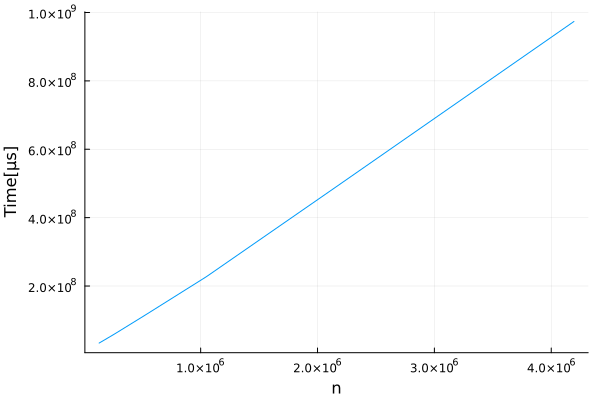
\includegraphics[width=10pc]{figures/experiments/scale_n.png}
  }
  \caption{ Linear runtime scaling }
  \label{scale_n}
\end{figure}

% TODO
% \subsubsection{Scaling with the number of dimensions}
% High dimensionality should affect the morton encoding since bit-interleaving scales
% linearly with the dimensions. The reordering should be affected slightly since each
% element


\subsubsection{Scaling with number of threads}
For uniformly distributed $n=10^6$ points of $d=10$ dimensions and a target tree of
$l=4$ levels, graph \ref{scale_t} suggests that the runtime of
\verb|AdaptiveHierarchicalRegularBinning.jl| drops exponatialy
with the number of threads.

\begin{figure}[!ht]
  \centerline{
    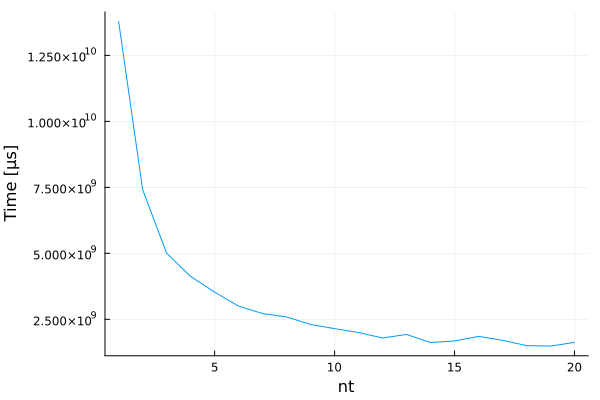
\includegraphics[width=10pc]{figures/experiments/scale_t.png}
  }
  \caption{ Parallelization scaling }
  \label{scale_t}
\end{figure}

We would expect that for a large enough number of threads the performance would worsen,
since the runtime complexity of the \verb|Countsort| algorithm suggests that if not
$n \gg t^2 \cdot r$ then the parallel variant is worse than the sequential one. Our
implementation gets around that limitation using the waterfall scheme for its
parallelization and thus for small sub-arrays the sequential variant for the
\verb|Countsort| is used.


\subsection{Point per node distribution}

\subsubsection{Uniform data 2 dimensions}

For uniformly distributed data we expect that each leaf node will contain
$n_{\textrm{leaf}}$ points.
$$n_{\textrm{leaf}} = \frac{n}{2^{l\cdot d}}$$

In this case $n = 10^5$, $d = 2$ and $l = 4$. So the expected number of points within a
node is $n_{\textrm{leaf}} = \frac{10^5}{2^{4\cdot 2}} =390.625$.

\begin{figure}[!ht]
  \centerline{
    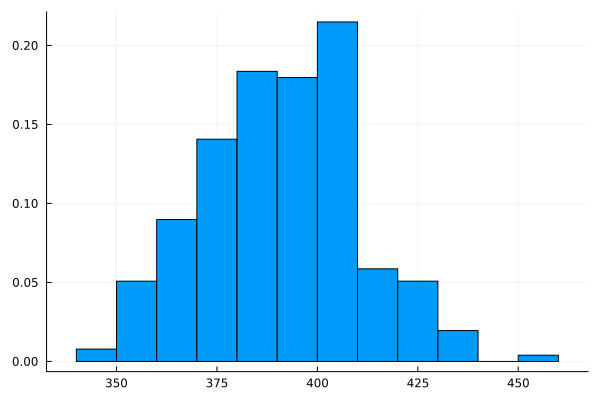
\includegraphics[width=10pc]{figures/experiments/uniform_2d/hist.png}
  }
  \caption{ Distribution of leaf node length }
  \label{uniform-2d-hist}
\end{figure}

Graph \ref{uniform-2d-hist} agrees with the theoreticaly expected value, although there
is some variance. This is to be expected, increasing the number of points will reduce
the variance then the histogram will tend more to the expected singular value.


\subsubsection{Curse of high dimensionality}
For $n=10^5$ uniformly distributed points we computed the average number of points in a
leaf node of the tree. The graph \ref{b_vs_d} shows that for increasingly higher
dimensional spaces the data get exponatialy sparser.

\begin{figure}[!ht]
  \centerline{
    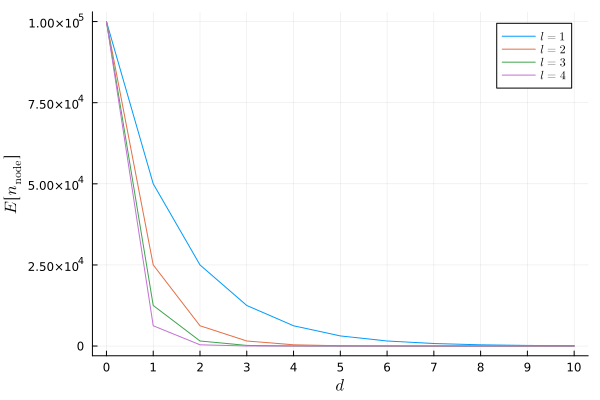
\includegraphics[width=10pc]{figures/experiments/b_vs_d.png}
  }
  \caption{ Exponential decrease of mean number of points per leaf node }
  \label{b_vs_d}
\end{figure}


\subsubsection{PBMC 30 dimensions}

The PBMC dataset exhibits outliers, which introduces challenges in the
normalization process. It causes the majority of data points to be clustered
into a single node for the first three levels of the tree. As depicted in
Figures \ref{pbmc-30-hist} (a), (b), and (c), the majority of points are
concentrated within a maximum of two nodes at these initial levels.
\\\\
However, the fourth and final level of the tree highlights the impact of the
dataset's high dimensionality. As indicated by Figure \ref{pbmc-30-hist} (d),
it becomes apparent that most points are now assigned to nodes with a length of
only $1$.

\begin{figure}[!ht]
  \centerline{
    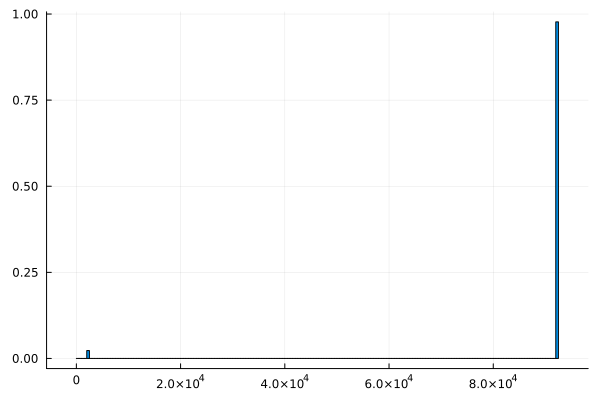
\includegraphics[width=10pc]{figures/experiments/pbmc_30/hist_1.png}
    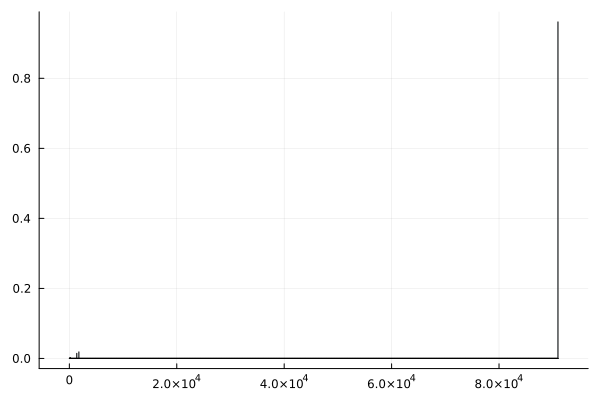
\includegraphics[width=10pc]{figures/experiments/pbmc_30/hist_2.png}
  }
  \centerline{
    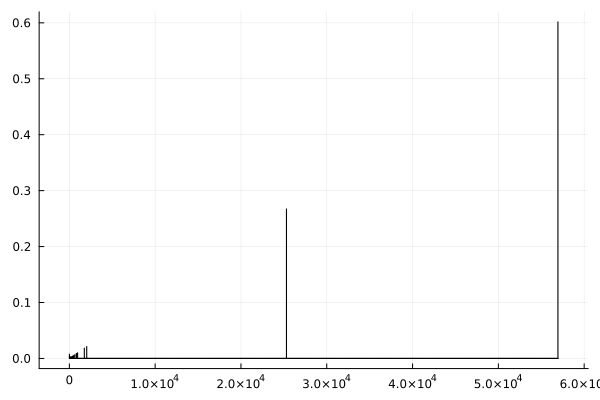
\includegraphics[width=10pc]{figures/experiments/pbmc_30/hist_3.png}
    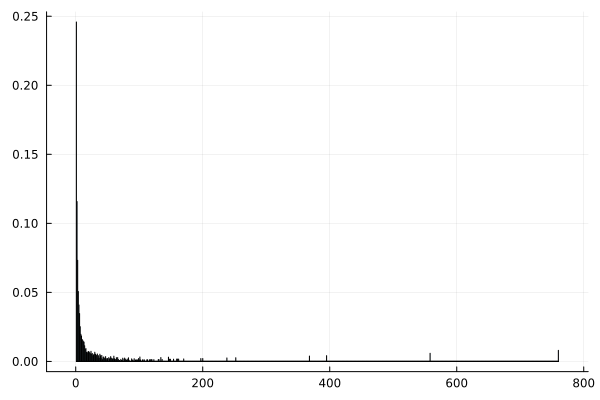
\includegraphics[width=10pc]{figures/experiments/pbmc_30/hist_4.png}
  }

  \caption{
    30-Dimensional PBMC data distribution of leaf node length per leaf for tree
    level (a) 1 (b) 2 (c) 3 (d) 4.
  }
  \label{pbmc-30-hist}
\end{figure}


\subsubsection{MNIST 30 dimensions}

Unlike the PBMC dataset, the MNIST dataset does not exhibit significant
outliers. As a result, the distribution between the leaf nodes in the tree
becomes more uniform. Figure \ref{mnist-30-hist} (a) reveals that a majority of
points are concentrated within leaf nodes that possess sufficiently large
lengths. This favorable grouping indicates a more balanced distribution of data
points.
\\\\
However, as we progress to lower levels of the tree, the impact of the
dataset's high dimensionality becomes apparent. Consequently, the points become
exponentially sparser, leading to the formation of singleton leaf nodes.
This observation is clearly demonstrated in Figure \ref{mnist-30-hist} (b).

\begin{figure}[!ht]
  \centerline{
    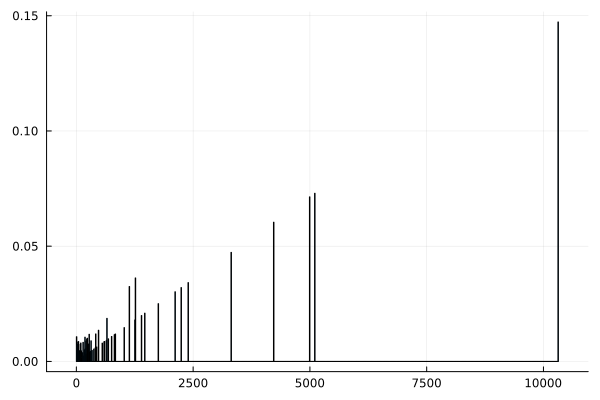
\includegraphics[width=10pc]{figures/experiments/mnist_30/hist_1.png}
    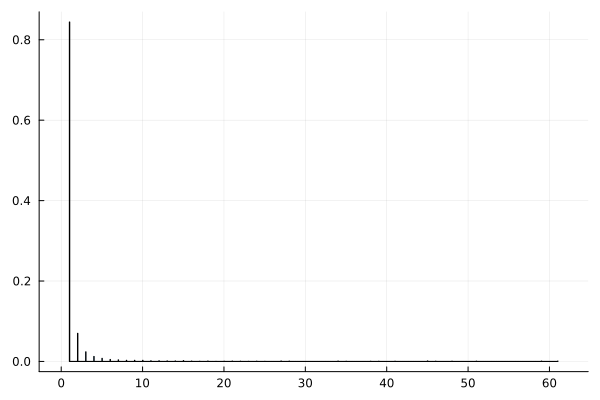
\includegraphics[width=10pc]{figures/experiments/mnist_30/hist_2.png}
  }

  \caption{
    30-Dimensional MNIST data distribution of leaf node length per point for
    tree level (a) 1 (b) 2
  }
  \label{mnist-30-hist}
\end{figure}

Figure \ref{mnist-30-hist-th} indicates that adjusting the \verb|Small|
threshold to approximately $10000$ causes a shift in nodes from the region of
$\geq 10000$ to the histogram's small node region, while leaving the rest of
the nodes intact. This outcome is expected because nearly all points in the
$\geq 10000$ region are mapped to a singleton node in the subsequent recursion.

\begin{figure}[!ht]
  \centerline{
    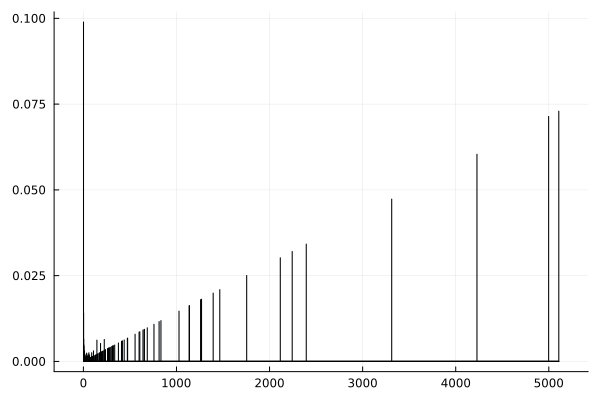
\includegraphics[width=10pc]{figures/experiments/mnist_30/hist_3.png}
  }

  \caption{
    30-Dimensional MNIST data distribution of leaf node length per point for
    tree of max level 2. Using Small threshold of 10000.
  }
  \label{mnist-30-hist-th}
\end{figure}

% **************GENERATED FILE, DO NOT EDIT**************

\bibliographystyle{juliacon}
\bibliography{ref.bib}




\end{document}

% Inspired by the International Journal of Computer Applications template
